\subsection{Dynamic Models}

Dynamic models illustrate the dynamic behavior of the system and the interactions between its components.
Different dynamic model types include UML activity, state chart, communication, and sequence diagrams.
Because of the large number of components in FLOps, this section focuses on sequence diagrams to cover a large set of significant interactions.

This subsection depicts the necessary interactions for a typical FLOps project.
We use many abstractions and depict the absolute base case for an FLOps project to reduce complexities and improve readability.
The base case aims to showcase a project workflow from the ground up.
That means that no code, data, or images are present yet.
This base case terminates after successful training.
It has no post-training steps, such as building and deploying an inference server.
FLOps management consists of multiple components.
For simplicity's sake, these components are grouped into one. 
The same applies to multiple worker nodes and edge devices.
To improve readability and comprehension we split up the project into stages.



\subsubsection{0. Preparation}

\begin{figure}[t]
    \begin{adjustwidth}{-0.1\paperwidth}{-0.1\paperwidth}
        \centering
        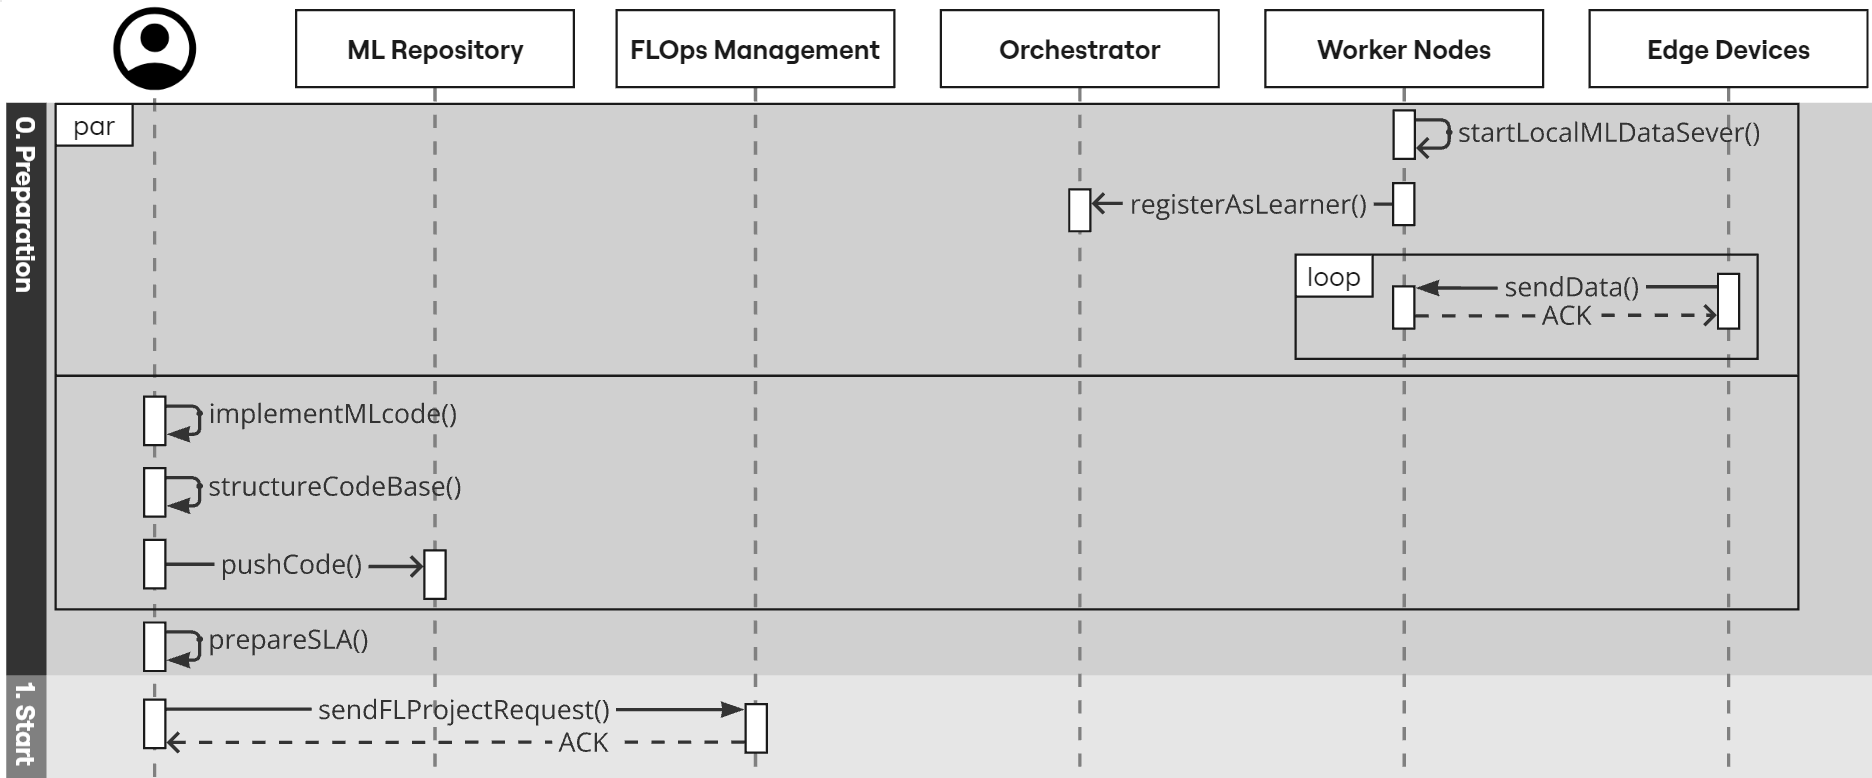
\includegraphics[width=0.9\paperwidth]{uml_sequence_init.png}
        \caption{FLOps Preparation - UML Sequence Diagram}
        \label{fig:uml_sequence_init}
    \end{adjustwidth}
\end{figure}

Figure \ref{fig:uml_sequence_init} is a UML sequence diagram depicting the initial steps before a FLOps project can start.
Two different sets of sequences can occur independently or in parallel with each other.
Before FLOps can run properly, FL worker nodes need to register with the orchestrator and stay available.
Only a subset of worker nodes are intended to be capable of performing ML training.
Worker nodes that should participate as learners must inform the orchestrator accordingly and start the provided ML data server locally.
This server accumulates training data locally for later training.
This process has to occur before training begins.
Otherwise, not enough or no data will be available for training.
Edge devices or other nearby data sources should send their data to these designated learner nodes.
The infrastructure provider has to ensure that these worker nodes are appropriately protected and trustworthy.
Once these steps are completed, FLOps should have access to available data-rich orchestrated worker nodes.

The second set of tasks that should occur before using FLOps is for users to prepare their ML code.
They should implement their ML code and structure it as required for FLOps.
This code must be available via an accessible git-based repository.
If the user is satisfied with his codebase, he can prepare his SLA.
(We discuss the SLA in detail in the implementation chapter.)
After both sequences have been completed, the user can send his SLA to the FLOps management API and request the start of a new FLOps project.

\subsubsection{1. Project Start}

Figure \ref{fig:uml_sequence_project_start} shows the main sequence of steps from starting a new FLOps project to deploying an image builder service.
The light blue activity bars mean that FLOps creates a new object inside the manager context, independent of the orchestrator and deployed components.
Management objects hold stateful information and are not run or used for computational workloads.
This split is necessary for the FLOps management to keep track of ongoing processes, retain memory, and handle unique custom requirements independent of and unavailable in the orchestrator.
Each colored or white rectangle on a lifeline inside the central UML sequence diagram corresponds to a specific functionality.
When this functionality terminates, the bar stops as well.
Usually, sequence diagrams show concrete instances of classes as actors.
We use abstract actors to optimize the page space and allow further abstractions and simplifications.
For example, the lifeline of an observatory app inside the orchestrator could be a separate actor.
However, this would lead to redundancy and verbosity between the orchestrator and observatory actors.
Instead, these modified graphs show the lifeline of FLOps components on the right side.
The color and dotted lines help to link those concepts together.
Light rose orchestrator actions symbolize a service being appended to an existing application.

The FLOps Management registered the new project request and extracted the SLA.
Firstly, the FLOps management creates a new observatory for the user inside the FLOps management context.
The management requests to create a corresponding app inside the orchestrator.
The same applies to the actual FLOps project.
When these two parent applications exist, the management will create the first service.
The management requests the creation of the project observer as a service inside the observatory application.
The management then requests to deploy an instance of this service on a worker node to the orchestrator.
Now, the user can access this project observer service at any time to observe the progress of his project.

The FLOps management checks if its image registry already contains images that match the requested ML repository.
For this, the management contacts the ML repository to check its latest state.
In this example, the registry is empty.
Therefore, new images are required.

\begin{figure}[t]
    \begin{adjustwidth}{-0.2\paperwidth}{-0.2\paperwidth}
        \centering
        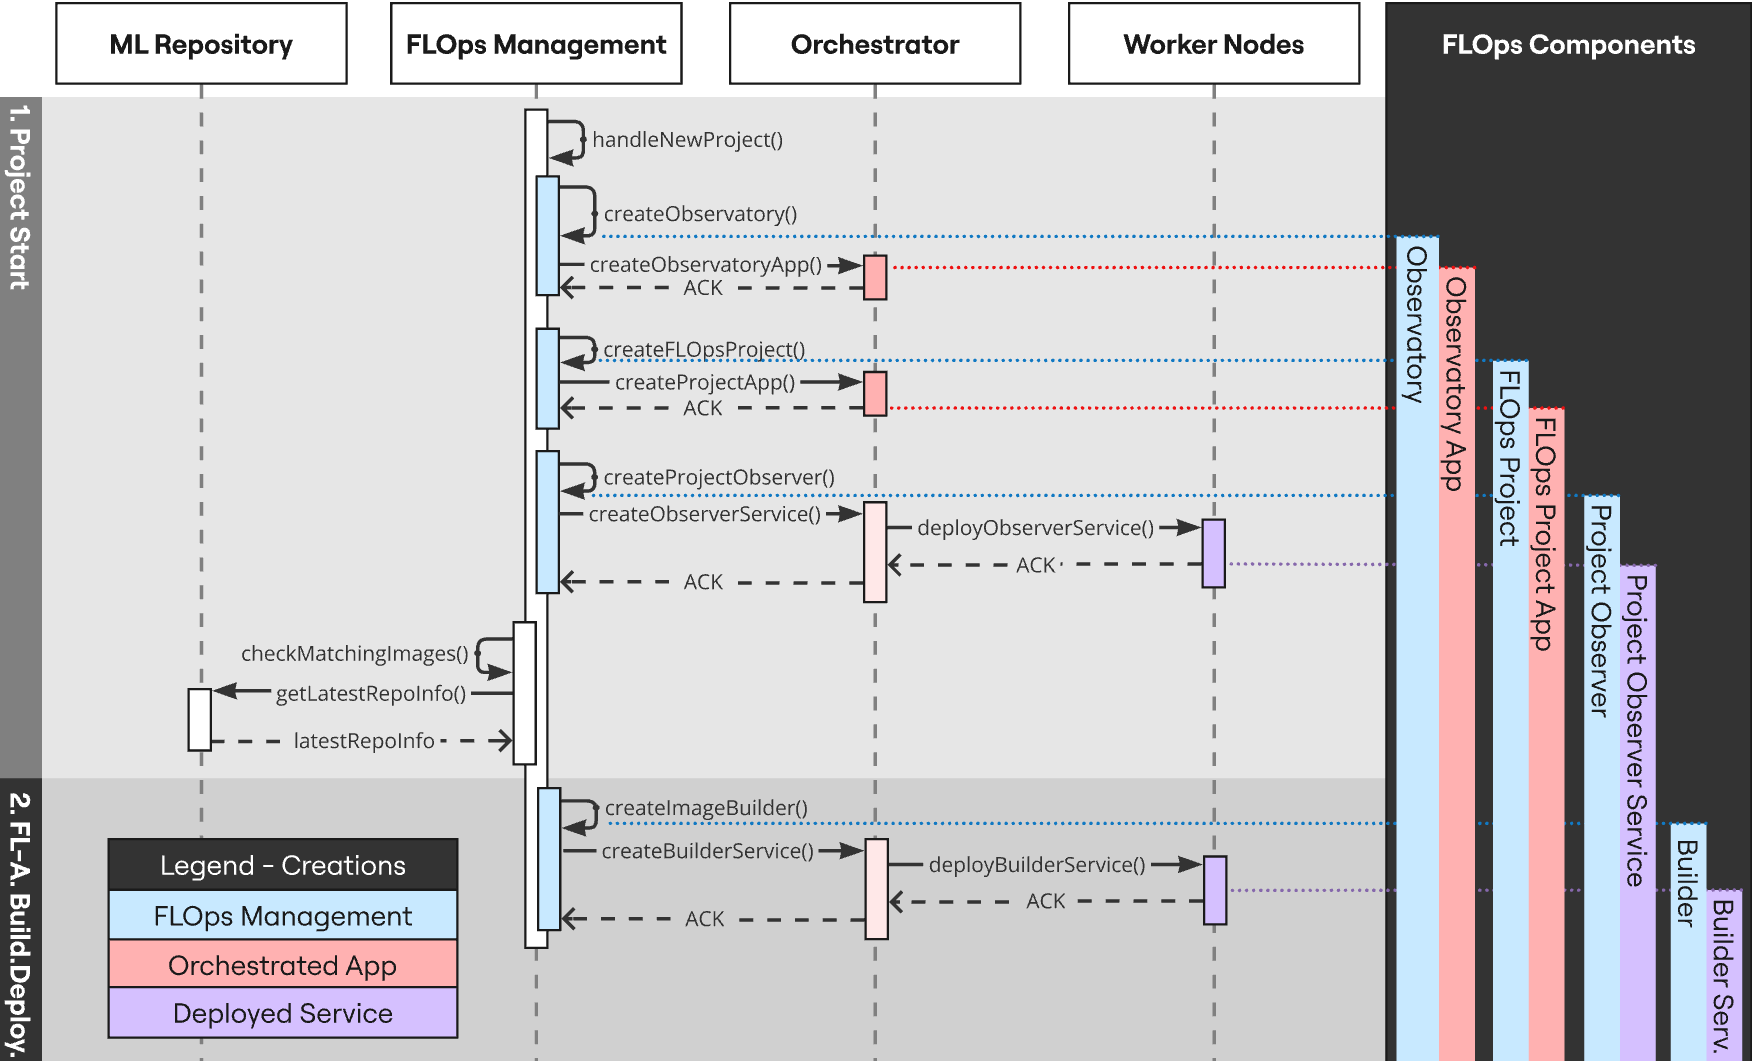
\includegraphics[width=0.95\paperwidth]{uml_sequence_diagram_project_start.png}
        \caption{FLOps Project Start - UML Sequence Diagram}
        \label{fig:uml_sequence_project_start}
    \end{adjustwidth}
\end{figure}

\subsubsection{2. FL-Actors Image-Builder Deployment}
The management creates a new image builder service and deploys it similarly to the project observer.

\subsubsection{3. FL-Actors Image Build}

\begin{figure}[t]
    \begin{adjustwidth}{-0.2\paperwidth}{-0.2\paperwidth}
        \centering
        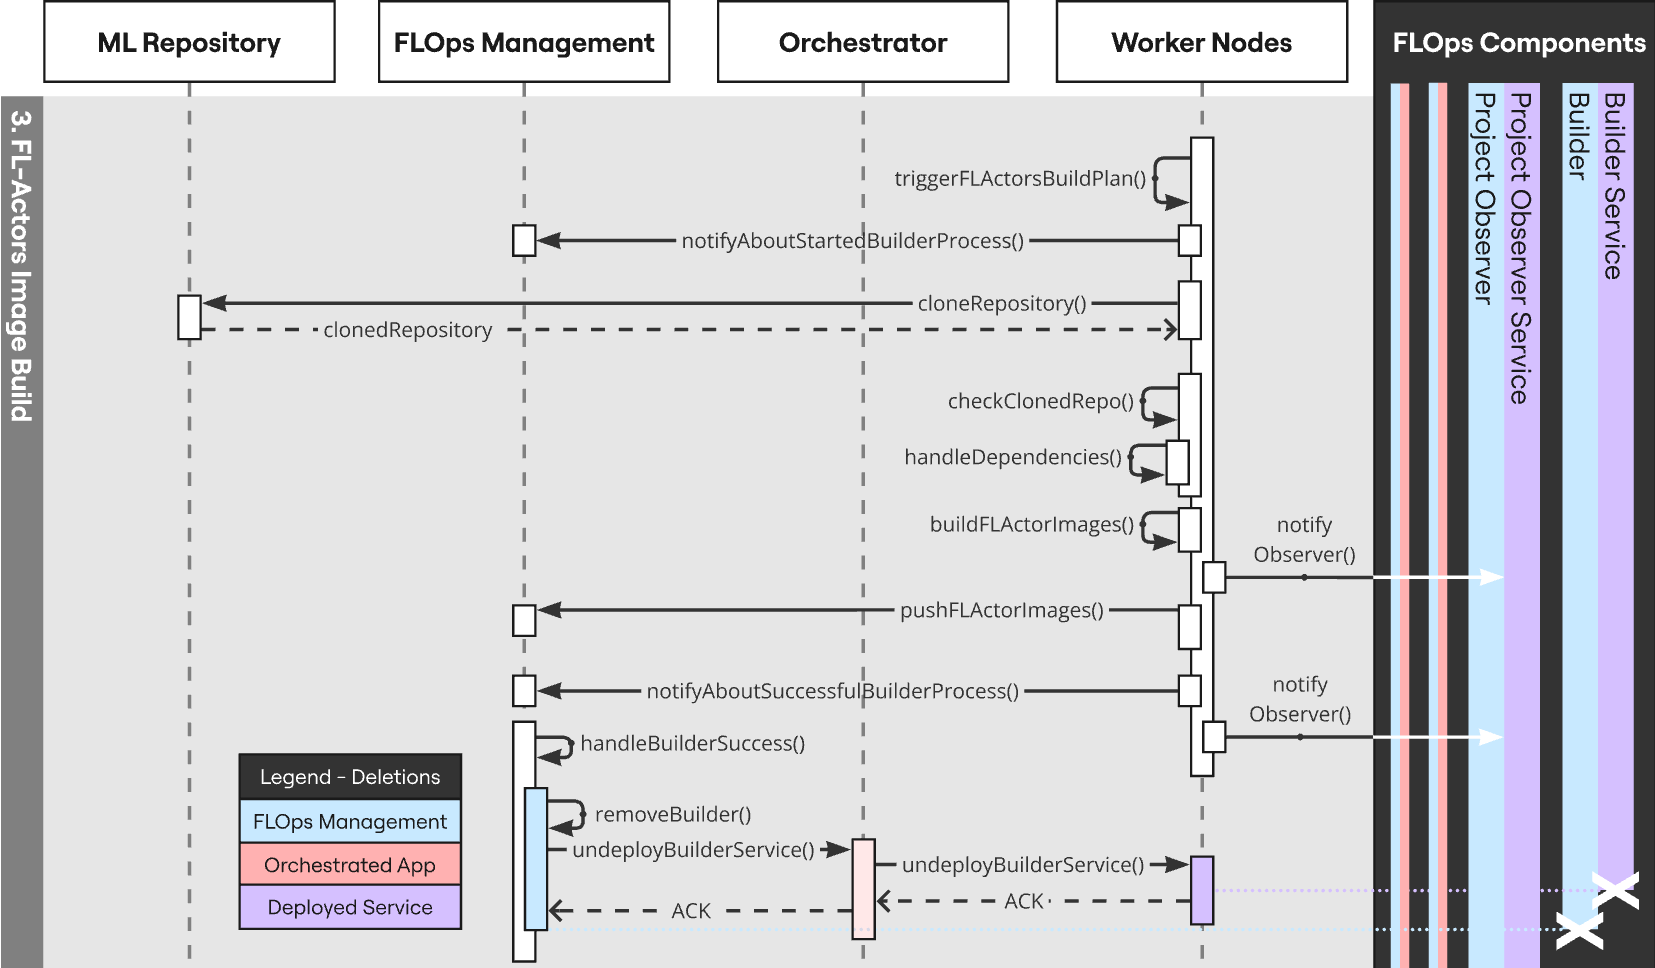
\includegraphics[width=0.95\paperwidth]{uml_sequence_actor_builder.png}
        \caption{FLOps Image Builder Processes - UML Sequence Diagram}
        \label{fig:uml_sequence_builder}
    \end{adjustwidth}
\end{figure}

Figure \ref{fig:uml_sequence_builder} shows the interactions necessary to augment user ML code into FL-enabled containerized images.
Once the builder service is deployed, it executes the build plan for actor images.
FL actors are the aggregator(s) and learners.
The builder service notifies the management about a successful start of this process.
It proceeds by cloning the ML repository and checks if it complies with FLOps requirements.
The builder also checks if the dependencies are sound.
When these build prerequisites are met, the builder continues to build the aggregator and learner images.
(Concrete details about this build process are available in the implementation chapter.)

Afterward, the builder notifies the project observer to inform the user about the successful build.
Note that the sequence model action lengths do not correspond to their actual duration.
Short rectangles visualize the build and push actions in the diagram, even though these two actions are by far the most time-consuming.

As the last build process step, the builder pushes these built images to the image registry hosted by the FLOps management.
After the successful push, the builder notifies the project observer and FLOps management of its successful completion.
The FLOps management catches this message and removes the builder from its own context and undeploys it from the orchestrator and worker.
Now that the FL actor images are ready, the training can begin.

\begin{figure}[p]
    \begin{adjustwidth}{-0.2\paperwidth}{-0.2\paperwidth}
        \centering
        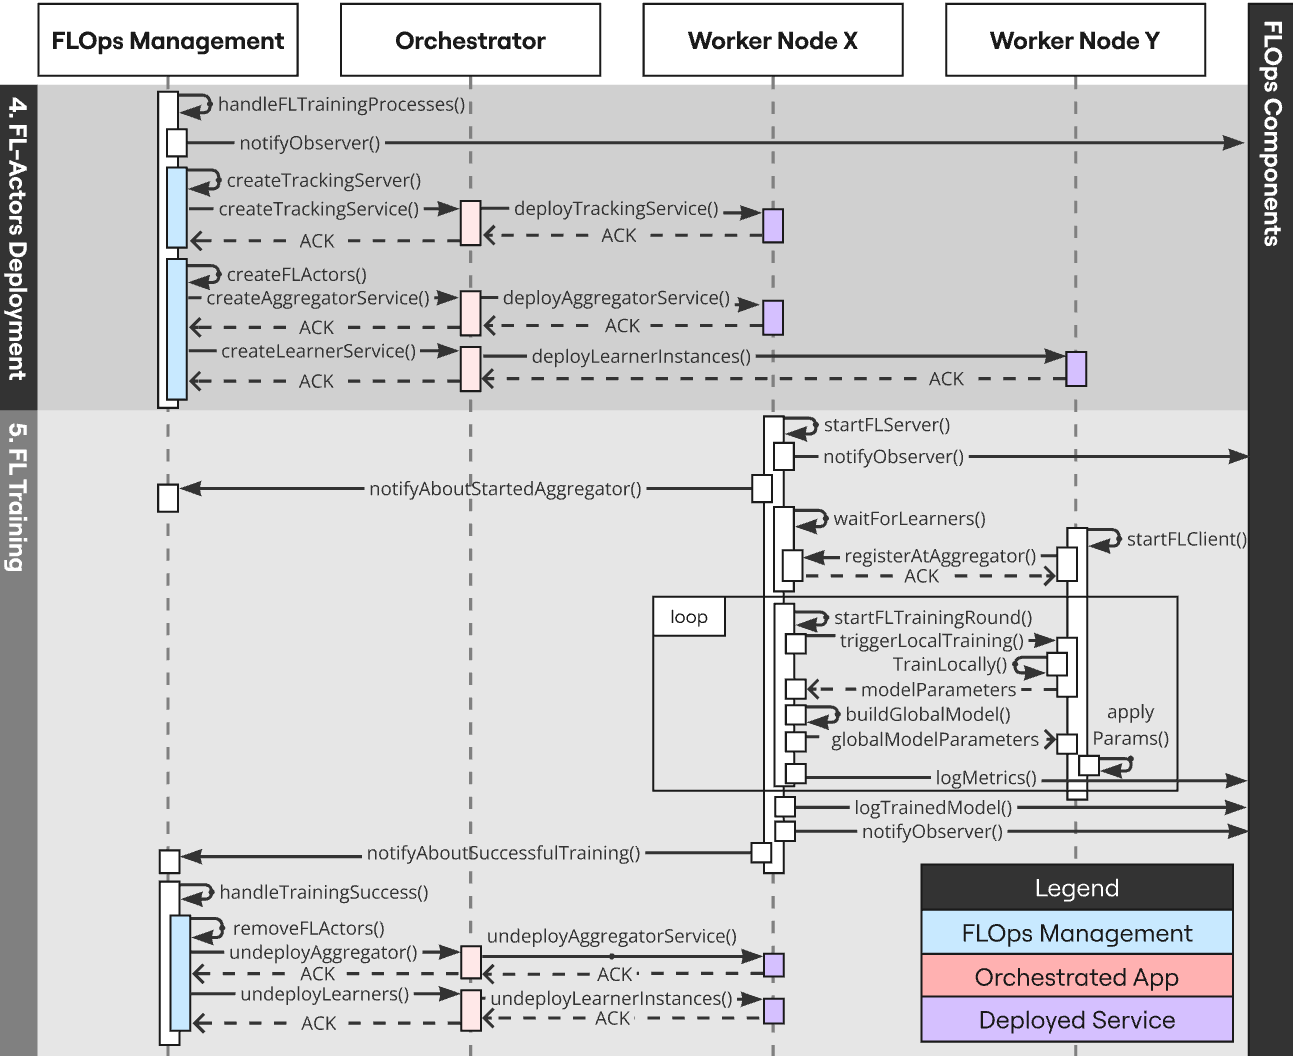
\includegraphics[width=0.95\paperwidth]{uml_sequence_training.png}
        \caption{FLOps FL Training Processes - UML Sequence Diagram}
        \label{fig:uml_sequence_training}
    \end{adjustwidth}
\end{figure}

Figure \ref{fig:uml_sequence_training} shows the necessary interactions that realize FL training under FLOps.
Note that the right side omits the previously depicted detailed FLOps component lifelines.
We collapse these details for this diagram because the depicted components and their lifetimes show similar behavior as the previous diagrams.
Arrows that point to the right mean that specific FLOps components are targeted.
They are not explicitly depicted to optimize readability and reduce verbosity.

\subsubsection{4. FL-Actors Deployment (Aggregator Deployment Stage)}
After building the required images, the FLOps management will start handling the FL training processes.
Firstly, it notifies the project observer that FL training will start shortly.
Secondly, it creates and deploys the tracking server that provides the GUI.
Users can access this GUI by following the link shown in the project observer or directly accessing the deployed tracking service, similarly to the project observer.
Note that there are several differences between the project observer and the GUI.
The project observer is a minimalistic way to inform the user about the current state and potential errors during the lifetime of an FLOps project.
The GUI is a standalone application that focuses on tracking the training results.

The FLOps management now creates and deploys the FL aggregator and learners.
It uses the previously built images for this.
Once the aggregator image is pulled and executed, it starts the FL server processes and notifies its watchers about its success.
The aggregator waits for learners to connect before starting the training.
In the meantime, the FL learner images were pulled and started.
Each learner starts its FL client activities, such as registering with its specified aggregator.

\subsubsection{5. FL Training}
Now that all FL actors are ready, the aggregator starts the first training round and triggers the learners.
The learners train their models with the local data from their worker node.
When completed, the learners will push their model parameters to the aggregator.
The aggregator fuses them into a new global model and returns the new global parameters to the learners.
The learners apply those to their local model to be ready to begin the next FL training round.
After each FL training round, the aggregator logs metrics, such as accuracy and loss, via the tracking server service.
The FLOps management stores the logged results.

After the last FL training round, the aggregator notifies its observers and logs the final trained model via the tracking service.
The aggregator only tracks the model a single time to avoid wasting bandwidth or storage.
Afterward, the aggregator and learner activities terminate.
Similarly to the builder's un-deployment process, the FLOps management registers the successful message and removes the FL actors.
With this, the core FLOps project is concluded.

\subsubsection{Further Stages}
Similarly, FLOps realizes more complex configurations, modes, or post-training steps.
For the post-training steps, the builder gets deployed again.
This time, it runs the trained model build plan and pulls the model from the FLOps management.
It pushes the built image back to the management image registry.
The inference service gets deployed similarly to the FL actors using the built trained model image.
